%%%%%%%%%%%%  Generated using docx2latex.com  %%%%%%%%%%%%%%

%%%%%%%%%%%%  v2.0.0-beta  %%%%%%%%%%%%%%

\documentclass[12pt]{report}
\usepackage{amsmath}
\usepackage{latexsym}
\usepackage{amsfonts}
\usepackage[normalem]{ulem}
\usepackage{soul}
\usepackage{array}
\usepackage{amssymb}
\usepackage{extarrows}
\usepackage{graphicx}
\usepackage[backend=biber,
style=numeric,
sorting=none,
isbn=false,
doi=false,
url=false,
]{biblatex}\addbibresource{bibliography-biblatex.bib}

\usepackage{subfig}
\usepackage{wrapfig}
\usepackage{wasysym}
\usepackage{enumitem}
\usepackage{adjustbox}
\usepackage{ragged2e}
\usepackage[svgnames,table]{xcolor}
\usepackage{tikz}
\usepackage{longtable}
\usepackage{changepage}
\usepackage{setspace}
\usepackage{hhline}
\usepackage{multicol}
\usepackage{tabto}
\usepackage{float}
\usepackage{multirow}
\usepackage{makecell}
\usepackage{fancyhdr}
\usepackage[toc,page]{appendix}
\usepackage[hidelinks]{hyperref}
\usetikzlibrary{shapes.symbols,shapes.geometric,shadows,arrows.meta}
\tikzset{>={Latex[width=1.5mm,length=2mm]}}
\usepackage{flowchart}\usepackage[paperheight=11.0in,paperwidth=8.5in,left=0.67in,right=0.68in,top=0.66in,bottom=1.55in,headheight=1in]{geometry}
\usepackage[utf8]{inputenc}
\usepackage[T1]{fontenc}
\TabPositions{0.5in,1.0in,1.5in,2.0in,2.5in,3.0in,3.5in,4.0in,4.5in,5.0in,5.5in,6.0in,6.5in,7.0in,}

\urlstyle{same}

\renewcommand{\_}{\kern-1.5pt\textunderscore\kern-1.5pt}

 %%%%%%%%%%%%  Set Depths for Sections  %%%%%%%%%%%%%%

% 1) Section
% 1.1) SubSection
% 1.1.1) SubSubSection
% 1.1.1.1) Paragraph
% 1.1.1.1.1) Subparagraph


\setcounter{tocdepth}{5}
\setcounter{secnumdepth}{5}


 %%%%%%%%%%%%  Set Depths for Nested Lists created by \begin{enumerate}  %%%%%%%%%%%%%%


\setlistdepth{9}
\renewlist{enumerate}{enumerate}{9}
		\setlist[enumerate,1]{label=\arabic*)}
		\setlist[enumerate,2]{label=\alph*)}
		\setlist[enumerate,3]{label=(\roman*)}
		\setlist[enumerate,4]{label=(\arabic*)}
		\setlist[enumerate,5]{label=(\Alph*)}
		\setlist[enumerate,6]{label=(\Roman*)}
		\setlist[enumerate,7]{label=\arabic*}
		\setlist[enumerate,8]{label=\alph*}
		\setlist[enumerate,9]{label=\roman*}

\renewlist{itemize}{itemize}{9}
		\setlist[itemize]{label=$\cdot$}
		\setlist[itemize,1]{label=\textbullet}
		\setlist[itemize,2]{label=$\circ$}
		\setlist[itemize,3]{label=$\ast$}
		\setlist[itemize,4]{label=$\dagger$}
		\setlist[itemize,5]{label=$\triangleright$}
		\setlist[itemize,6]{label=$\bigstar$}
		\setlist[itemize,7]{label=$\blacklozenge$}
		\setlist[itemize,8]{label=$\prime$}



 %%%%%%%%%%%%  Header here  %%%%%%%%%%%%%%


\pagestyle{fancy}
\fancyhf{}
\lfoot{ 
\vspace{\baselineskip}
Mentor: Prof. Jayprakash Lalchandani}
\renewcommand{\headrulewidth}{0pt}
\setlength{\topsep}{0pt}\setlength{\parindent}{0pt}

 %%%%%%%%%%%%  This sets linespacing (verticle gap between Lines) Default=1 %%%%%%%%%%%%%%


\renewcommand{\arraystretch}{1.3}


%%%%%%%%%%%%%%%%%%%% Document code starts here %%%%%%%%%%%%%%%%%%%%



\begin{document}
\begin{Center}
{\fontsize{23pt}{27.6pt}\selectfont Privacy Centered Android App : PrivacyWind}
\end{Center}

\vspace{\baselineskip}

\vspace{\baselineskip}
\begin{multicols}{2}
\begin{Center}
{\fontsize{14pt}{16.8pt}\selectfont \textit{Akash Jain}}
\end{Center}
\begin{Center}
{\fontsize{14pt}{16.8pt}\selectfont \textit{201701264}}
\end{Center}
\begin{Center}
{\fontsize{14pt}{16.8pt}\selectfont \textit{DA-IICT, Gandhinagar}}
\end{Center}
\begin{Center}
{\fontsize{14pt}{16.8pt}\selectfont \textit{Gujrat, India}}
\end{Center}
\begin{Center}
{\fontsize{14pt}{16.8pt}\selectfont \textit{201701264@daiict.ac.in}}
\end{Center}

\vspace{\baselineskip}
\begin{Center}
{\fontsize{14pt}{16.8pt}\selectfont \textit{Manas Kaul}}
\end{Center}
\begin{Center}
{\fontsize{14pt}{16.8pt}\selectfont \textit{201701417}}
\end{Center}
\begin{Center}
{\fontsize{14pt}{16.8pt}\selectfont \textit{DA-IICT, Gandhinagar}}
\end{Center}
\begin{Center}
{\fontsize{14pt}{16.8pt}\selectfont \textit{Gujrat, India}}
\end{Center}

\end{multicols}
\begin{Center}
{\fontsize{14pt}{16.8pt}\selectfont \textit{201701417@daiict.ac.in}}
\end{Center}
\begin{multicols}{2}

\vspace{\baselineskip}
\begin{justify}
{\fontsize{10pt}{12.0pt}\selectfont \textbf{Abstract - The PrivacyWind app is focused on android app development that helps users to control the permissions. The main objective of this application is to give users control over their phone’s installed application so that they can keep track of permissions accessed by these android apps.}\par}
\end{justify}

\vspace{\baselineskip}
\begin{Center}
\textbf{I. INTRODUCTION}
\end{Center}

\vspace{\baselineskip}
\begin{justify}
{\fontsize{10pt}{12.0pt}\selectfont Privacy nowadays is of utmost importance. Applications that you install on your smartphone are free but the real cost is your data. There are many applications on the play store that suspiciously try to access your smartphone’s data. There are plenty of people out there who would like to get their hands on this valuable asset that is your data.\par}
\end{justify}

\vspace{\baselineskip}
\begin{justify}
{\fontsize{10pt}{12.0pt}\selectfont \textit{A. MOTIVATION}}
\end{justify}
\begin{justify}
{\fontsize{10pt}{12.0pt}\selectfont When you grant your phones permission to a third party application, they can use it silently in the background without the user knowing about it. PrivacyWind is a privacy focused application that can help the user easily manage the permissions given to the third party applications and monitor them for any suspicious activity.The application also provides other features like permission manager, app search, app comparison, etc.\par}
\end{justify}
\begin{justify}
{\fontsize{10pt}{12.0pt}\selectfont PrivacyWind gives the user complete control over their smartphone's permissions and helps them protect their privacy.\par}
\end{justify}

\vspace{\baselineskip}
\begin{justify}
{\fontsize{10pt}{12.0pt}\selectfont \textit{B. PROPOSED SYSTEM}}
\end{justify}
\begin{justify}
{\fontsize{10pt}{12.0pt}\selectfont The proposed solution is an android application which gives users control over all the applications installed on their android device. The PrivacyWind app \par}
\end{justify}

\vspace{\baselineskip}
\begin{justify}
{\fontsize{10pt}{12.0pt}\selectfont gives users the ability to enable/disable any type of permissions. The app can also be used to search an application and view all the permissions before the user \par}
\end{justify}
\begin{justify}
{\fontsize{10pt}{12.0pt}\selectfont installs it on their device. The app is also capable to monitor and log when an app requests and access a permission so that it is easy to detect any suspicious \par}
\end{justify}
\begin{justify}
{\fontsize{10pt}{12.0pt}\selectfont behaviour.}
\end{justify}

\vspace{\baselineskip}
\begin{justify}
{\fontsize{10pt}{12.0pt}\selectfont \textit{C. RELATED WORK}}
\end{justify}
\begin{justify}
{\fontsize{10pt}{12.0pt}\selectfont Currently there are a few apps that provide the ability to manage permissions and log and keep track of permissions but they are not able to do what PrivacyWind can do. PrivacyWind keeps a detailed log of all the permissions. PrivacyWind has many features that are missing in these existing applications and many features that no application has like app search, app compare, watch list, etc.\par}
\end{justify}

\vspace{\baselineskip}
\setlength{\parskip}{12.0pt}
\begin{justify}
{\fontsize{10pt}{12.0pt}\selectfont Similar apps available :}
\end{justify}
\begin{justify}
{\fontsize{10pt}{12.0pt}\selectfont 1. Permission manager – Main purpose of this app is showing the user which permission is allowed or denied for any installed app on the device. When you want to toggle allow/deny, it redirects you to App information in settings where you can do so. Our app also supports this feature.\par}
\end{justify}
\begin{justify}
{\fontsize{10pt}{12.0pt}\selectfont 2. Access dots – Main purpose of this app is logging the permissions used by any installed app on the device. When the user allows monitoring, this app will check if any app is using Camera, Microphone or Location, it will show an indicator (colour dot) and make an entry in a logs file with permission name, app name and time when it’s used. Our app also supports this feature.\par}
\end{justify}
\begin{justify}
{\fontsize{10pt}{12.0pt}\selectfont Our app: PrivacyWind – Permission manager doesn’t have a feature of making logs and Access dots doesn’t have a feature of showing and toggling of permissions allow/deny for any installed app. There are also some other features that both applications don’t support which are mentioned below. \par}
\end{justify}
\begin{justify}
{\fontsize{10pt}{12.0pt}\selectfont Alert feature: Main purpose of our app is to alert users, if any installed is doing privacy breach through resources like Camera, Microphone or Location then app indicates it as suspicious activity and will make logs with red alert. So, the user can decide if he/she still wants to use an app which has done a privacy breach or to uninstall it.\par}
\end{justify}
\begin{justify}
{\fontsize{10pt}{12.0pt}\selectfont Rating feature: We have designed an algorithm which gets logs from all the Users of our apps. On the basis of logs, the algorithm does computation and assigns a rating out of 10 to apps. Higher the rating shows the app is more trustworthy and the lower rating indicates the app can be harmful to your privacy.\par}
\end{justify}
\begin{justify}
{\fontsize{10pt}{12.0pt}\selectfont Comparison feature: We can compare 2 or 3 apps from the same category on Google Play Store. Comparison will show which app is requiring which permissions if an app is being installed along with rating. So, User can decide which permissions he is okay to give and with the help of rating, User can choose the safest option to go with.\par}
\end{justify}

\vspace{\baselineskip}
\setlength{\parskip}{0.0pt}

\vspace{\baselineskip}
\begin{Center}
{\fontsize{10pt}{12.0pt}\selectfont \textbf{II. SYSTEM REQUIREMENTS}}
\end{Center}

\vspace{\baselineskip}
\begin{justify}
{\fontsize{10pt}{12.0pt}\selectfont \textit{A. HARDWARE REQUIREMENTS}}
\end{justify}
\begin{enumerate}
	\item {\fontsize{10pt}{12.0pt}\selectfont Smartphone Type : Android Device}
	\item {\fontsize{10pt}{12.0pt}\selectfont RAM : Minimum of 512 MB}
\end{enumerate}

\vspace{\baselineskip}
\begin{justify}
{\fontsize{10pt}{12.0pt}\selectfont \textit{B. SOFTWARE REQUIREMENTS}}
\end{justify}
\begin{enumerate}
	\item {\fontsize{10pt}{12.0pt}\selectfont Operating System : Minimum Android 8 Oreo}
	\item {\fontsize{10pt}{12.0pt}\selectfont Google Play Store to install app}
\end{enumerate}

\vspace{\baselineskip}

\vspace{\baselineskip}

\vspace{\baselineskip}
\begin{Center}
{\fontsize{10pt}{12.0pt}\selectfont \textbf{III. FEATURES $\&$  FUNCTIONALITY}}
\end{Center}

\vspace{\baselineskip}
\begin{justify}
{\fontsize{10pt}{12.0pt}\selectfont The PrivacyWind app has three major features:}
\end{justify}

\vspace{\baselineskip}
\begin{justify}
{\fontsize{10pt}{12.0pt}\selectfont A. PERMISSION MANAGER}
\end{justify}
\begin{justify}
{\fontsize{10pt}{12.0pt}\selectfont \tab The app gets the information about all the installed apps. This list of apps is then displayed to the user. Users can then choose from the list and select an app to see the list of permissions that the app has access to. A switch is also displayed which the user can use to toggle the permission from allowed to denied And vice versa. After the android 8.0 version, Android OS has reserved the action of toggling permission to allow/deny to itself. So if User wants to toggle, we redirect him to App information in Settings. Where User can toggle any permission to allow/deny state. \par}
\end{justify}

\vspace{\baselineskip}
\begin{justify}
{\fontsize{10pt}{12.0pt}\selectfont B. APP SEARCH}
\end{justify}
\begin{justify}
{\fontsize{10pt}{12.0pt}\selectfont \tab The user is provided with a search box in which the user can search any application name. The user is then shown a list of apps matching the search term. The user can then select an app to get the list of permissions for that app or add the app to a compare list. The compare list compares the apps based on the permissions requested by them.\par}
\end{justify}

\vspace{\baselineskip}
\begin{justify}
{\fontsize{10pt}{12.0pt}\selectfont C. APP MONITOR}
\end{justify}
\begin{justify}
\tab {\fontsize{10pt}{12.0pt}\selectfont This feature is used to monitor and keep track of all the permissions that a third party application might use or access while the app is running. This would help the user keep track of permission accessed by the application and also helps in detection of any suspicious activity. All the permissions accessed activity is logged and the user can easily view these logs. These activity logs are automatically shared with the server for better experience. When the user wants to use this feature for the first time, App by default adds all installed Applications in monitoring watch-list. Then the user can remove and add any app according to his choice.\par}
\end{justify}

\vspace{\baselineskip}

\vspace{\baselineskip}
\begin{Center}
{\fontsize{10pt}{12.0pt}\selectfont \textbf{IV. DESIGN}}
\end{Center}

\vspace{\baselineskip}
\begin{justify}
{\fontsize{10pt}{12.0pt}\selectfont A. DESIGN APPROACH}
\end{justify}
\begin{justify}
{\fontsize{10pt}{12.0pt}\selectfont \tab This project is based on the functional design approach. Following is the activity diagram for the application:\par}
\end{justify}

\vspace{\baselineskip}


%%%%%%%%%%%%%%%%%%%% Figure/Image No: 1 starts here %%%%%%%%%%%%%%%%%%%%

\begin{figure}[H]
	\begin{Center}
		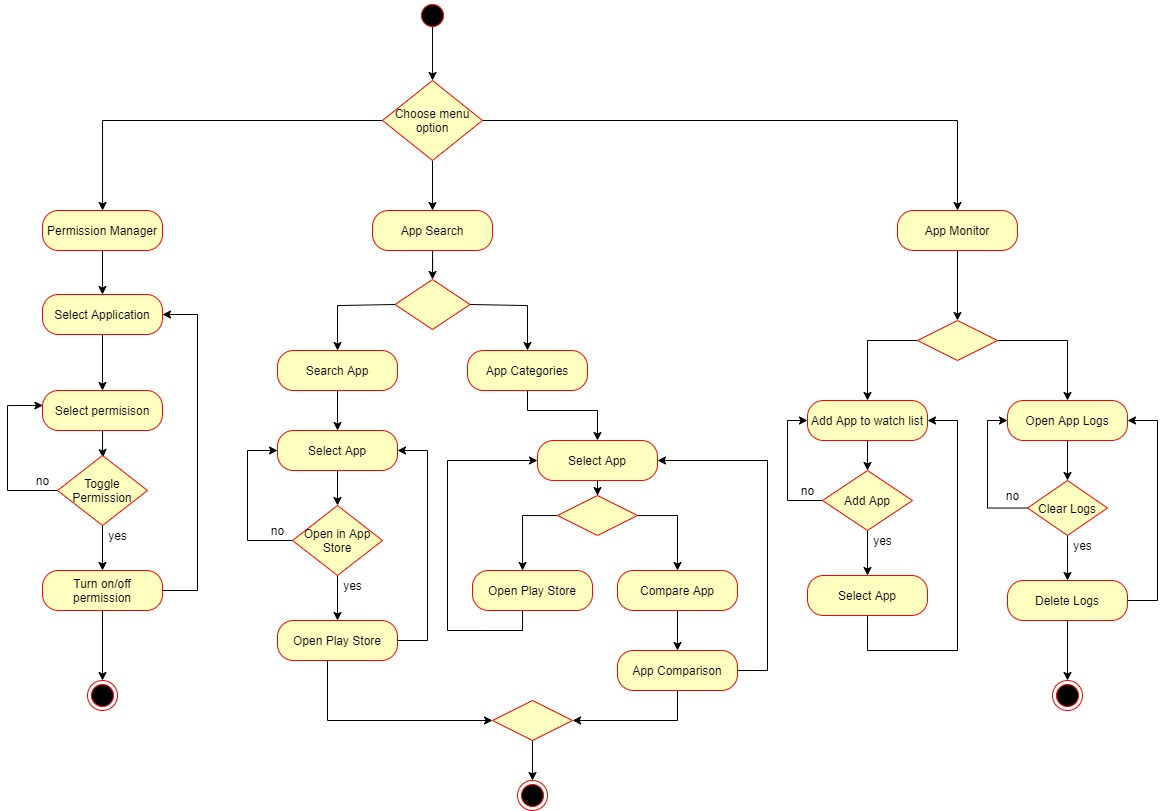
\includegraphics[width=3.45in,height=2.4in]{./media/image9.jpg}
	\end{Center}
\end{figure}


%%%%%%%%%%%%%%%%%%%% Figure/Image No: 1 Ends here %%%%%%%%%%%%%%%%%%%%


\vspace{\baselineskip}\begin{Center}
{\fontsize{10pt}{12.0pt}\selectfont Fig. 1 : Activity Diagram for PrivacyWind}
\end{Center}

\vspace{\baselineskip}
\begin{justify}
{\fontsize{10pt}{12.0pt}\selectfont B. DETAILED DESIGN}
\end{justify}
\begin{enumerate}
	\item {\fontsize{10pt}{12.0pt}\selectfont App List}
\begin{justify}
{\fontsize{10pt}{12.0pt}\selectfont A list of apps is shown to the user with the app name and app icon. This is a clickable tile which would then show the permissions requested by the selected app.\par}
\end{justify}

\vspace{\baselineskip}


%%%%%%%%%%%%%%%%%%%% Figure/Image No: 2 starts here %%%%%%%%%%%%%%%%%%%%

\begin{figure}[H]
	\begin{Center}
		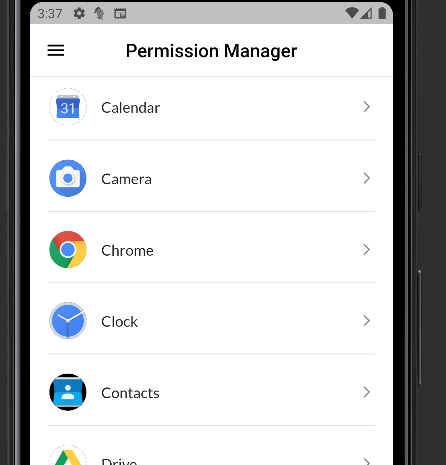
\includegraphics[width=2.72in,height=2.69in]{./media/image1.png}
	\end{Center}
\end{figure}


%%%%%%%%%%%%%%%%%%%% Figure/Image No: 2 Ends here %%%%%%%%%%%%%%%%%%%%


\vspace{\baselineskip}
\vspace{\baselineskip}
\begin{Center}
{\fontsize{10pt}{12.0pt}\selectfont Fig. 2 : App List}
\end{Center}

\vspace{\baselineskip}
	\item {\fontsize{10pt}{12.0pt}\selectfont Permission Details}
\begin{justify}
{\fontsize{10pt}{12.0pt}\selectfont A list of permissions is displayed to the user along with a switch which indicates whether the permission is given access to or not. The permission can be given/revoked access by just clicking on the switch.\par}
\end{justify}

\vspace{\baselineskip}


%%%%%%%%%%%%%%%%%%%% Figure/Image No: 3 starts here %%%%%%%%%%%%%%%%%%%%

\begin{figure}[H]
	\begin{FlushRight}		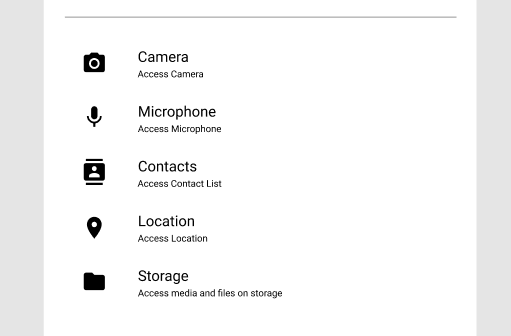
\includegraphics[width=2.89in,height=2.06in]{./media/image3.png}
	\end{FlushRight}\end{figure}


%%%%%%%%%%%%%%%%%%%% Figure/Image No: 3 Ends here %%%%%%%%%%%%%%%%%%%%


\vspace{\baselineskip}\begin{Center}
{\fontsize{10pt}{12.0pt}\selectfont Fig. 3 : Permissions List}
\end{Center}

\vspace{\baselineskip}
	\item {\fontsize{10pt}{12.0pt}\selectfont Search App}
\begin{justify}
{\fontsize{10pt}{12.0pt}\selectfont A Search box is provided which can be used to search an application. Users can input a search term and top ten relevant apps are displayed to the user. All these are clickable tiles which show the permissions requested by the app.\par}
\end{justify}

\vspace{\baselineskip}


%%%%%%%%%%%%%%%%%%%% Figure/Image No: 4 starts here %%%%%%%%%%%%%%%%%%%%

\begin{figure}[H]
	\begin{Center}
		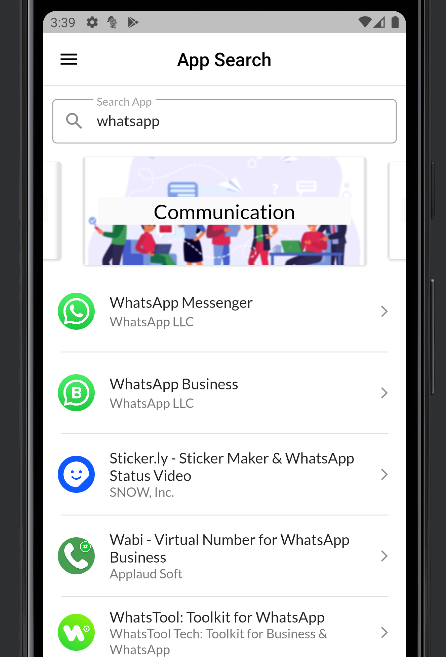
\includegraphics[width=2.32in,height=2.76in]{./media/image5.png}
	\end{Center}
\end{figure}


%%%%%%%%%%%%%%%%%%%% Figure/Image No: 4 Ends here %%%%%%%%%%%%%%%%%%%%


\vspace{\baselineskip}
\vspace{\baselineskip}
\begin{Center}
{\fontsize{10pt}{12.0pt}\selectfont Fig. 4 : Search page}
\end{Center}

\vspace{\baselineskip}
	\item {\fontsize{10pt}{12.0pt}\selectfont App Categories}
\begin{justify}
{\fontsize{10pt}{12.0pt}\selectfont A list of categories is displayed which can be used to get a list of items falling under a similar category. Users can also choose to compare the apps in a category.\par}
\end{justify}

\vspace{\baselineskip}


%%%%%%%%%%%%%%%%%%%% Figure/Image No: 5 starts here %%%%%%%%%%%%%%%%%%%%

\begin{figure}[H]
	\begin{Center}
		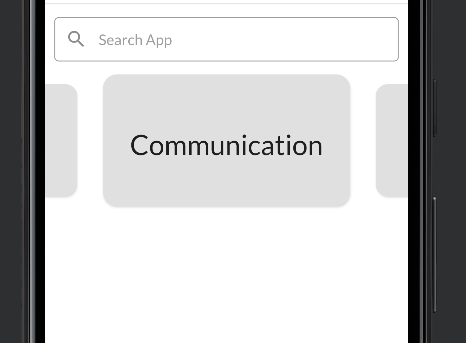
\includegraphics[width=2.61in,height=1.2in]{./media/image7.png}
	\end{Center}
\end{figure}


%%%%%%%%%%%%%%%%%%%% Figure/Image No: 5 Ends here %%%%%%%%%%%%%%%%%%%%


\vspace{\baselineskip}\begin{Center}
{\fontsize{10pt}{12.0pt}\selectfont Fig. 5 : Search Categories}
\end{Center}

\vspace{\baselineskip}
	\item {\fontsize{10pt}{12.0pt}\selectfont App Compare}
\begin{justify}
{\fontsize{10pt}{12.0pt}\selectfont Users have an option to compare applications. When comparing applications a list of permissions used is displayed.\par}
\end{justify}

\vspace{\baselineskip}


%%%%%%%%%%%%%%%%%%%% Figure/Image No: 6 starts here %%%%%%%%%%%%%%%%%%%%

\begin{figure}[H]
	\begin{Center}
		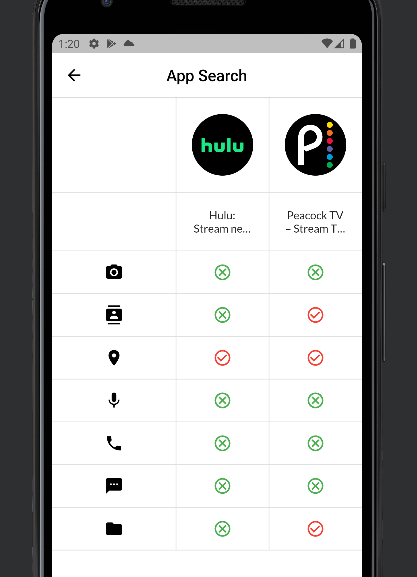
\includegraphics[width=1.79in,height=2.66in]{./media/image8.png}
	\end{Center}
\end{figure}


%%%%%%%%%%%%%%%%%%%% Figure/Image No: 6 Ends here %%%%%%%%%%%%%%%%%%%%


\vspace{\baselineskip}
\vspace{\baselineskip}
\begin{Center}
{\fontsize{10pt}{12.0pt}\selectfont Fig. 6 : Compare page}
\end{Center}

\vspace{\baselineskip}
	\item {\fontsize{10pt}{12.0pt}\selectfont Watchlist}
\begin{justify}
{\fontsize{10pt}{12.0pt}\selectfont Users can add applications to the watchlist to }
\end{justify}
\begin{justify}
{\fontsize{10pt}{12.0pt}\selectfont monitor the permissions used.}
\end{justify}

\vspace{\baselineskip}


%%%%%%%%%%%%%%%%%%%% Figure/Image No: 7 starts here %%%%%%%%%%%%%%%%%%%%

\begin{figure}[H]
	\begin{Center}
		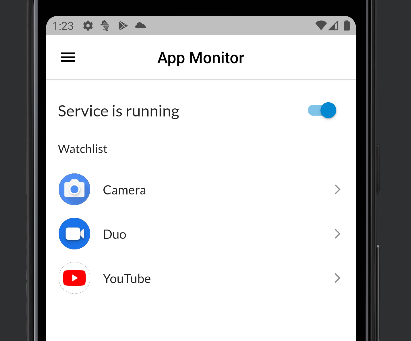
\includegraphics[width=2.58in,height=1.86in]{./media/image4.png}
	\end{Center}
\end{figure}


%%%%%%%%%%%%%%%%%%%% Figure/Image No: 7 Ends here %%%%%%%%%%%%%%%%%%%%


\vspace{\baselineskip}\begin{Center}
{\fontsize{10pt}{12.0pt}\selectfont Fig. 7 : Search page}
\end{Center}

\vspace{\baselineskip}

\vspace{\baselineskip}
	\item {\fontsize{10pt}{12.0pt}\selectfont App Logs}
\end{enumerate}
\begin{justify}
{\fontsize{10pt}{12.0pt}\selectfont When the user turns on the monitoring service and when an application accesses any permission, this is recorded along with the timestamp and displayed when the user opens the application to check the details. If there is any suspicious activity recorder, the user is notified.\par}
\end{justify}


%%%%%%%%%%%%%%%%%%%% Figure/Image No: 8 starts here %%%%%%%%%%%%%%%%%%%%

\begin{figure}[H]
	\begin{Center}
		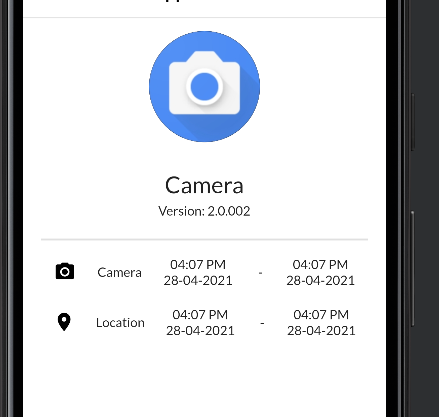
\includegraphics[width=2.82in,height=2.62in]{./media/image6.png}
	\end{Center}
\end{figure}


%%%%%%%%%%%%%%%%%%%% Figure/Image No: 8 Ends here %%%%%%%%%%%%%%%%%%%%


\vspace{\baselineskip}\begin{Center}
{\fontsize{10pt}{12.0pt}\selectfont Fig. 8 : App Logs}
\end{Center}

\vspace{\baselineskip}

\vspace{\baselineskip}

\vspace{\baselineskip}
\begin{Center}
{\fontsize{10pt}{12.0pt}\selectfont \textbf{V. IMPLEMENTATION}}
\end{Center}

\vspace{\baselineskip}
\setlength{\parskip}{12.0pt}
\begin{justify}
{\fontsize{10pt}{12.0pt}\selectfont 1. Introduction to programming languages }
\end{justify}
\begin{justify}
{\fontsize{10pt}{12.0pt}\selectfont 1.1 Java}
\end{justify}
\begin{justify}
{\fontsize{10pt}{12.0pt}\selectfont \ \ \ \ \ \ \  As the project is developing an operating-system related app, the very best option for language is java with very well-built libraries. Java addressed drawbacks of C, C++ and became the popular language. [x] the language is so easy to learn and implement. Java can be used in various kinds of applications like Web, Desktop, Mobile, Big data etc. With the help of various libraries, application services and graphics libraries, Java can provide powerful features. Java supports OOPS (Object Oriented Programming) concepts and is more competent as they are scalable, extensible, and flexible. it has a platform independence feature including any virtual machines (Write Once Read Everywhere), as in no need to write the code for different OS as the Java Compilers convert the java source files to bytecode and this could be interpreted by any machine and the actual code is compiled irrespective of any machine, OS. It is more secured as the compilers are designed efficiently to figure out any kind of errors.\par}
\end{justify}
\begin{justify}
{\fontsize{10pt}{12.0pt}\selectfont 1.2 Dart}
\end{justify}
\begin{justify}
{\fontsize{10pt}{12.0pt}\selectfont \ \ \ \ \ \ \  \tab We have used Flutter for better UI experience. Flutter uses Dart as Dart allows Flutter to avoid the need for a separate declarative layout language like JSX and XML. The layout of Dart is declarative programmatic, and it makes it easy for developers to read and visualize it very easily and effortlessly. In addition to that, it makes it easy for Flutter to provide additional tooling as the layout is in one language and a commonplace. The language has a clean and incredibly powerful syntax that sets ideal conditions for creating a clear architecture and design of the application. And Syntax Structure is so easy to learn that programmers with a little experience of any popular languages like Java, C$\#$ , Typescript can switch to Dart smoothly and start using it.\par}
\end{justify}
\begin{justify}
{\fontsize{10pt}{12.0pt}\selectfont 2. Introduction to IDE’s, Tools and Technologies - }
\end{justify}
\begin{justify}
{\fontsize{10pt}{12.0pt}\selectfont 2.1 Android Studio}
\end{justify}
\begin{justify}
{\fontsize{10pt}{12.0pt}\selectfont \ \ \ \ \ \ \  \tab Exclusively designed for developing Android Applications, Android Studio consists of all Android SDK tools to design, develop, maintain, test, debug and publish an android app. Android Studio uses Gradle which is an advanced build toolkit, to automate and manage the build process, while allowing developers to define flexible custom build configurations. Android Studio provides advance code completion which is better compared to Eclipse. Android Studio uses module structure to manage multiple projects. We can define gradle build files for all code modules which start their own dependencies. It also supports Git as a version control system to maintain code changes. After the completion of the project, the whole application can be put as an .APK (android package) file, which we can run in android phone and use the application.\par}
\end{justify}
\begin{justify}
{\fontsize{10pt}{12.0pt}\selectfont 2.2 Android Software Development Kit (SDK):}
\end{justify}
\begin{justify}
{\fontsize{10pt}{12.0pt}\selectfont Android SDK includes libraries, a debugger, a handset emulator, documentation and sample code. Which helps to avoid writing a lot of codes and make application development smoother and faster.\par}
\end{justify}
\begin{justify}
{\fontsize{10pt}{12.0pt}\selectfont 2.3 Android Debug Bridge (ADB):}
\end{justify}
\begin{justify}
{\fontsize{10pt}{12.0pt}\selectfont \ \ \ \ \ \ \  \tab Android SDK uses ADB, a command line tool which helps in communicating with a device. By using ADB commands we can Install and Debug android apps on a device, track the system logs and perform a variety of commands on a device from Unix shell.\par}
\end{justify}
\begin{justify}
{\fontsize{10pt}{12.0pt}\selectfont  2.4 Gradle Build:}
\end{justify}
\begin{justify}
{\fontsize{10pt}{12.0pt}\selectfont \ \ \ \ \ \ \  \tab Gradle is Build system which automates various app development phases including code compilation, testing, deployment and converting code into .dex files and compressing all of them into a single .apk file, which is our application. We need to configure the project/module by mentioning all the supported jar files, build tools, set defalutconfigs includes applicationId, minSDKVersion, targetSDKVersion, VersionName etc., to ensure app is compatible with device/emulator. Gradle is similar to maven, a helping tool to maintain java repositories.\par}
\end{justify}
\begin{justify}
{\fontsize{10pt}{12.0pt}\selectfont 2.5 SQLite Database}
\end{justify}
\begin{justify}
{\fontsize{10pt}{12.0pt}\selectfont \ \ \ \ \ \ \  \tab Android Supports inbuilt database SQLite which can be very useful for small applications. We can perform any CRUD (Create, Read, Update, Delete) operations on SQLite Database. In order to access this database, we don’t require any kind of connections like we do in JDBC, ODBC.\par}
\end{justify}
\begin{justify}
{\fontsize{10pt}{12.0pt}\selectfont 3.\  Rating algorithm:}
\end{justify}
\begin{justify}
{\fontsize{10pt}{12.0pt}\selectfont \ \ \ \ \ \ \  \tab We have implemented a rating algorithm which is running on the backend. With the User’s consent, we ask the user to share permission logs details. As of now we have covered three permissions Camera, Microphone and Location, and all the 3 permissions contribute equally (33$\%$ ) in final rating. We have taken 3 situations into consideration to rate any application. First in which Permission was not asked but still was being used then the app gets the lowest score (0 out of 3.33) for violated permission. Second in which Permission was asked, but usage was not allowed by User and still app used then it gets a medium score (1.33 out of 3.33) for violated permission. And Third situation in which Permission was asked and usage was also allowed by User, so in this case the app acted as it should be and it gets the highest score (3.33 out of 3.33) for particular permission. By considering these 3 scenarios, Algorithm rates applications and helps to identify if an app is Trustworthy, or we should avoid it.\par}
\end{justify}
\begin{justify}
{\fontsize{10pt}{12.0pt}\selectfont 4.\ \ Server : We have used Node JS and Express to develop backend, and MongoDB as a database. Database is deployed on Mongo Atlas, which is a very popular, scalable and Trustworthy cloud database service. For hosting backend we used cloud platform Heroku, which is a scalable and self-maintained Application Hosting Platform. As of now for testing purposes free service works perfectly fine but once the application is published on Google Play Store, Heroku paid  service is a great choice. The server can handle queries regarding fetching details of any app available on Google Play Store, Comparing apps. Server also runs a rating algorithm (discussed in sec 3) which gets permission logs from clients and by computation it assigns rating to the app which decides how safe the app is. This working for the same is shown in Fig. N9 .\par}
\end{justify}


%%%%%%%%%%%%%%%%%%%% Figure/Image No: 9 starts here %%%%%%%%%%%%%%%%%%%%

\begin{figure}[H]
	\begin{Center}
		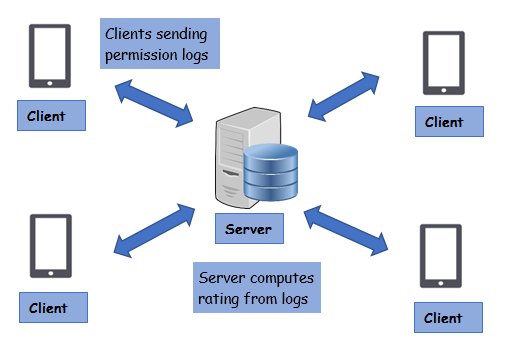
\includegraphics[width=3.45in,height=2.31in]{./media/image2.png}
	\end{Center}
\end{figure}


%%%%%%%%%%%%%%%%%%%% Figure/Image No: 9 Ends here %%%%%%%%%%%%%%%%%%%%


\vspace{\baselineskip}\begin{Center}
{\fontsize{10pt}{12.0pt}\selectfont Fig. 9 :Fetching logs and rating of application}
\end{Center}

\vspace{\baselineskip}
\setlength{\parskip}{0.0pt}

\vspace{\baselineskip}

\vspace{\baselineskip}
\begin{Center}
{\fontsize{10pt}{12.0pt}\selectfont \textbf{VI. CONCLUSION}}
\end{Center}

\vspace{\baselineskip}
\setlength{\parskip}{12.0pt}
\begin{justify}
{\fontsize{10pt}{12.0pt}\selectfont This BTech Project provided us an exposure to Flutter and Android Development. As our Application is very close to Android OS, we got to explore Android OS and in general whole Android development (Services, PackageManagers, Accessibility Feature, permissions, etc) in a more detailed way. Our app helps users to monitor behaviour of installed apps on the phone. And reports if any suspicious activity is detected like permission is not allowed still resource is used. Also, based on Rating User can compare apps from the same category and choose a very safe option. Overall, we have made an app which will help users to become more aware about Security while using different apps on a daily basis.\par}
\end{justify}

\vspace{\baselineskip}
\setlength{\parskip}{0.0pt}

\vspace{\baselineskip}
\begin{Center}
{\fontsize{10pt}{12.0pt}\selectfont \textbf{VII. FUTURE WORK}}
\end{Center}

\vspace{\baselineskip}
\begin{justify}
{\fontsize{10pt}{12.0pt}\selectfont The PrivacyWind app has a lot of important features that one could use to better keep track of their privacy. Still there are few features that can be added:\par}
\end{justify}
\begin{enumerate}
	\item {\fontsize{10pt}{12.0pt}\selectfont Monitoring every type of permission. Currently the app is capable of monitoring only three major permissions - Camera, Microphone and Location. Other permissions like SMS, Contacts, etc can also be added to improve the features.\par}

\vspace{\baselineskip}
	\item {\fontsize{10pt}{12.0pt}\selectfont Feature to install and use an application in a virtual environment so that the user can first get an idea of the security and privacy features of the application before he/she installs it to their smartphone. Currently there are two options for this : \par}
\begin{justify}
{\fontsize{10pt}{12.0pt}\selectfont (1) Installing and running the application locally. This option will require elevated root access from users device which if done wrong might lead to corrupting the android device. and\par}
\end{justify}
\begin{justify}
{\fontsize{10pt}{12.0pt}\selectfont (2) Installing and running applications on cloud. This can only be done using a desktop and this is generally used by companies wanting to test their applications on different devices.\par}
\end{justify}

\vspace{\baselineskip}
	\item {\fontsize{10pt}{12.0pt}\selectfont Currently the latest Android OS does not allow to automate permission change. If in future this changes, a feature can be added to automatically toggle permission preference without redirection to settings page.\par}

\vspace{\baselineskip}
	\item {\fontsize{10pt}{12.0pt}\selectfont A feature to detect any other suspicious or malicious activity by an application that might put the privacy of the user at risk.\par}
\end{enumerate}

\vspace{\baselineskip}

\vspace{\baselineskip}

\vspace{\baselineskip}

\vspace{\baselineskip}
\begin{Center}
{\fontsize{10pt}{12.0pt}\selectfont \textbf{VIII. REFERENCES}}
\end{Center}

\vspace{\baselineskip}
\begin{thebibliography}{99}
\bibitem{item1}
{\fontsize{10pt}{12.0pt}\selectfont Flutter Docs}
\begin{justify}
\href{https://flutter.dev/docs}{\textcolor[HTML]{1155CC}{\ul{https://flutter.dev/docs}}}
\end{justify}
\bibitem{item2}
{\fontsize{10pt}{12.0pt}\selectfont Android Docs \href{https://developer.android.com/docs}{\textcolor[HTML]{1155CC}{\ul{https://developer.android.com/docs}}}}
\bibitem{item3}
{\fontsize{10pt}{12.0pt}\selectfont Safe Dot Github \href{https://github.com/kamaravichow/safe-dot-android}{\textcolor[HTML]{1155CC}{\ul{https://github.com/kamaravichow/safe-dot-android}}}}
\bibitem{item4}
{\fontsize{10pt}{12.0pt}\selectfont Accessibility Docs \href{https://developer.android.com/guide/topics/ui/accessibility/service#java}{\textcolor[HTML]{1155CC}{\ul{https://developer.android.com/guide/topics/ui/accessibility/service$\#$ java}}}}
\bibitem{item5}
{\fontsize{10pt}{12.0pt}\selectfont Platform Integration \href{https://flutter.dev/docs/development/platform-integration/platform-channels}{\textcolor[HTML]{1155CC}{\ul{https://flutter.dev/docs/development/platform-integration/platform-channels}}}}
\bibitem{item6}
{\fontsize{10pt}{12.0pt}\selectfont Flutter Packages}
\end{thebibliography}
\href{https://pub.dev/}{\textcolor[HTML]{1155CC}{\ul{https://pub.dev/}}}

\vspace{\baselineskip}

\end{multicols}
\printbibliography
\end{document}